\documentclass{ximera}


\preambleinput{../preamble}

\title{Complex Numbers From Different Angles}

\begin{document}
\begin{abstract}
In this activity we will investigate complex multiplication.
\end{abstract}
\maketitle




\begin{question} Consider the innocent little equation:
\[
x^3 -1 = 0
\]
How many solutions does it have? What are they? Plot them on the
complex plane below.
\[
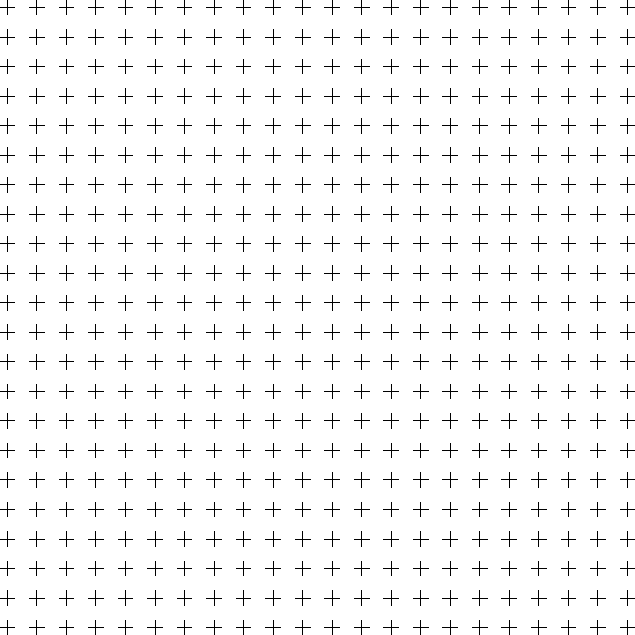
\includegraphics{complexPlane.pdf}
\]
\end{question}

\begin{question}
Thinking about your work above, see if you can solve:
\[
x^4 -1 = 0
\]
Plot the solutions on the complex plane below.
\[
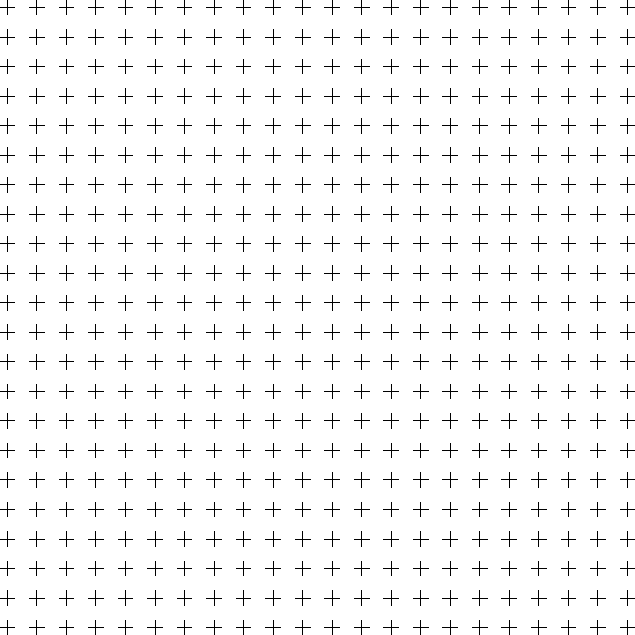
\includegraphics{complexPlane.pdf}
\]
\end{question}


\begin{question}
Suppose I told you that:
\begin{align*}
\sin(x) &= x - \frac{x^3}{3!} + \frac{x^5}{5!} - \frac{x^7}{7!} + \dots + \frac{(-1)^n x^{2n+1}}{(2n+1)!} + \cdots \\
\cos(x) &= 1 - \frac{x^2}{2!} + \frac{x^4}{4!} - \frac{x^6}{6!} + \dots + \frac{(-1)^n x^{2n}}{(2n)!} + \cdots \\
e^x &= 1 + x + \frac{x^2}{2!} + \frac{x^3}{3!} + \frac{x^4}{4!} + \dots + \frac{x^n}{n!} + \cdots 
\end{align*}
Explain why we say:
\[
e^{x\cdot i} = \cos(x) + i \sin(x)
\]
\end{question}

\begin{question}
 This is Euler's famous formula:
\[
e^{\pi \cdot i } + 1 = 0
\]
Use the questionlem above to explain why it is true.
\end{question}

\begin{question}
What does all this have to do with De Moivre's Theorem?
\end{question}

\begin{question}
How can you use this to take the $n$th root of a complex number?
\end{question}
\end{document}
